


\section{Introduction} 
This report revists the \emph{period enforcer} algorithm proposed by Rajkumar \cite{Raj:suspension1991} to handle self-suspending real-time tasks. The report briefly reviews the period enforcer algorithm, explains its underlying assumptions and limitations, and discusses how it may be analyzed to correctly determine the schedulability of self-suspending sporadic real-time tasks subject to period enforcement. 

The main contributions of this report are two observations that have not been previously reported in the real-time literature:

\begin{enumerate}
	\item period enforcement can render self-suspending tasks sets unschedulable that are schedulable otherwise (i.e., period enforcement can induce deadline misses); and
	\item with current techniques, schedulability analysis of the period enforcer algorithm requires a task set transformation that is subject to exponential time complexity.
\end{enumerate}

\subsection{Preliminaries}

To date, the real-time literature on self-suspending tasks has focused on two task models: the \emph{dynamic} and the \emph{segmented} (or \emph{multi-segment}) self-suspension model. 
The dynamic self-suspension sporadic task model characterizes each
task $\tau_i$ as a $4$-tuple $(C_i,S_i,T_i,D_i)$: 
$C_i$ denotes the upper bound on the total execution time of any job of $\tau_i$,
$S_i$ denotes the upper bound on the total self-suspension time of any job of $\tau_i$,
$T_i$ denotes the minimum inter-arrival time (or period) of $\tau_i$, and $D_i$ is the relative deadline. The dynamic self-suspension model does not impose a bound on the maximum number of self-suspensions, nor does it make any assumptions as to where during a job's execution self-suspensions occur.

In contrast, the segmented sporadic task model extends the above $4$-tuple by characterizing each self-suspending task as a (fixed) finite linear sequence of computation and suspension intervals. These intervals are represented as a tuple
$(C_{i}^1,S_{i}^1,C_{i}^2,S_{i}^2,...,S_{i}^{m_i-1},C_{i}^{m_i})$, which is composed of $m_i$ computation segments separated by $m_i-1$ suspension intervals. For the simplicity of presentation, we assume that a task $\tau_i$ always starts with a computation segment. The arguments can be easily extended to handle tasks that start with self-suspensions.

The advantage of the dynamic model is that it is more flexible since it does not impose any assumptions on control flow. The advantage of the segmented model is that is allows for more accurate analysis. The period enforcer algorithm and its analysis fundamentally applies (only) to the segmented model.

The central notation in Rajkumar's analysis~\cite{Raj:suspension1991} is a \emph{deferrable task}, which matches our notion of multi-segment tasks.  Specifically, Rajkumar states that:
\begin{quote}
With deferred execution, a task $\tau_i$ can execute its $C_i$ units of execution in discrete amounts $C_i^1, C_i^2$, $\ldots$ with suspension in between $C_i^j$ and $C_i^{j+1}$. \cite[Section 3]{Raj:suspension1991}\footnote{The notation has been altered here for the sake of consistency.} 
\end{quote}
%
Central to Rajkumar's analysis~\cite{Raj:suspension1991} is a \emph{task set transformation} that splits each deferrable task with multiple segments into a corresponding number of single-segment deferrable tasks.  In the words of Rajkumar~\cite[Section 3]{Raj:suspension1991}:

\begin{quote}
	 Without any loss of generality, we shall assume that a task $\tau_i$ can defer its entire execution time but not parts of it. That is, a task $\tau_i$ executes for $C_i$ units with no suspensions once it begins execution. Any task that does suspend after it executes for a while can be considered to be two or more tasks each with its own worst-case execution time. The only difference is that if a task $\tau_i$ is split into two tasks $\tau_i'$ followed by $\tau_i''$, then $\tau_i''$ has the same deadlines as $\tau_i{{'}}$. 
\end{quote}
%
In other words, the transformation can be understood as splitting each self-suspending task into a matching number of non-self-suspending sporadic tasks subject to \emph{release jitter}, which can be easily analyzed with classic fixed-priority response-time analysis~\cite{ABRTW:93}.

It is well known that uncontrolled deferred execution (i.e, release jitter) can impose a scheduling penalty because of the potential for ``back-to-back'' execution~\cite{ABRTW:93}. That is, if a job of a deferrable task that maximally defers its execution is directly followed by a job that executes immediately without deferring its execution, then lower-priority tasks may suffer increased interference. 

The purpose of the period enforcer algorithm is to reduce such penalties for lower-priority tasks without detrimentally affecting the schedulability of self-suspending, higher-priority tasks. The latter aspect --- no detrimental effects for self-suspending tasks --- is captured concisely by Theorem 5 in the original analysis of the period enforcer algorithm \cite{Raj:suspension1991}.
\begin{quote}
{\bf Theorem 5}: A deferrable task that is schedulable under its worst-case conditions is also schedulable under the period enforcer algorithm.  \cite{Raj:suspension1991}
\end{quote}

\subsection{Questions answered in this report}

Theorem 5 in \cite{Raj:suspension1991} provides a very positive result for the analysis of deferrable task sets subject to period enforcement: if the corresponding transformed task set can be shown to be schedulable under fixed-priority scheduling using \emph{any} applicable analysis, then the period enforcer algorithm also yields a correct schedule. 

However, note that Theorem 5 in \cite{Raj:suspension1991} applies only to the \emph{transformed} task set: recall that, in the original analysis~\cite{Raj:suspension1991}, deferrable tasks are assumed to defer their entire execution time either completely or not at all (but not parts of it).  Therefore, if we would like to use the period enforcer algorithm to handle segmented self-suspending task sets, we first have to answer the following question: ``\emph{Given a set of sporadic segmented self-suspending tasks, what is the corresponding set of (single-segment) deferrable tasks?}'' That is, how do we convert given self-suspension segments into equivalent bounds on release jitter such that we may apply Theorem 5 to conclude that the system remains schedulable despite period enforcement? 




In this report, which is motivated by the fact that the original proposal \cite{Raj:suspension1991} does not provide an answer to this central question, 
we make two pertinent observations.
\begin{enumerate}
	\item There exist sporadic segmented self-suspending task sets that are schedulable under fixed-priority scheduling without any enforcement, but the corresponding schedule by using the period enforcer algorithm is not feasible. This shows that Theorem 5 in \cite{Raj:suspension1991} has to be  used with care --- it may be applied only in the context of the transformed single-segment deferrable task set, and not in the context of the original segmented self-suspending task set.

	\item Deriving a single-segment deferrable task set corresponding to a given set of sporadic segmented self-suspending tasks in polynomial time is an open problem. Recent findings by Nelissen et al. \cite{ecrts15nelissen} can be applied, but their method takes exponential time.
\end{enumerate}

\section{Period Enforcement Can Induce Deadline Misses}
\label{sec:unschedulable}

In this section, we demonstrate with an example that there exist sporadic  segmented self-suspending task sets that both \textbf{(i)} are schedulable \emph{without} period enforcement and \textbf{(ii)} are not schedulable with period enforcement.

Consider a task system with $2$ tasks. Let $\tau_1$ denote a sporadic task without self-suspensions and parameters $C_1 = 2$ and $T_1=D_1=10$, and let $\tau_2$ denote a self-suspending task consisting of two segments with parameters  $C_{2,1} = 1$,  $S_{2,1} = 6$, $C_{2,2}=1$, and $ T_2=D_2=11$. Suppose that we use the rate-monotonic priority assignment, i.e., $\tau_1$ has higher priority than $\tau_2$. This task set is schedulable without any enforcement since at most one computation segment of a job of $\tau_2$ can be delayed by $\tau_1$: 
\begin{itemize}
	\item if the first segment of a job of $\tau_2$ is interfered with by $\tau_1$, then the second segment resumes at most after $9$ time units after the release of the job and the response time of task $\tau_2$ is hence $10$; otherwise,
	\item  if the first segment of a job of $\tau_2$ is not interfered with by $\tau_1$, then the second segment resumes at most $7$ time units after the release of the job and hence the  response time of task $\tau_2$ is at most $10$ even if the second segment is interfered with by $\tau_1$.
\end{itemize}


Let's release these two tasks periodically, starting from time $0$. The fixed-priority schedule is presented in Figure \ref{fig:example-original}.
The period enforcer algorithm determines for each segment (i.e., for each converted single-segment deferrable task) an \emph{eligibility time}. If a segment resumes (i.e., a job of a single-segment deferrable task arrives) before its eligibility time, the execution of the segment (i.e., the single-segment job) is delayed until the eligibility time is reached.

Let $ET_{2,j}^1$ and $ET_{2,j}^2$ denote the eligibility times of the first and second segment, respectively, of the $j^{\mathrm{th}}$ job of $\tau_2$. Further, let $a^1_{2,j}$ and $a^2_{2,j}$ denote the arrival times\footnote{A segment \emph{arrives} when it becomes available for execution. The first segment arrives immediately when the job is released; the segment arrives when the job resumes from its self-suspension.} of the job's first and second segment, respectively.  Finally, let $\mathit{busy}(\tau_2, t')$ denote the last time that a level-2 busy interval began on or prior to time $t'$. According to Section 3.1 in \cite{Raj:suspension1991}, the period enforcer algorithm then defines the segment eligibility times as
\begin{align*}
	ET_{2,j}^1 & = \max\left(ET_{2,j-1}^1 + T_2,\ \mathit{busy}(\tau_2, a^1_{2,j})\right)  \text{ and }
\\
	ET_{2,j}^2 & = \max\left(ET_{2,j-1}^2 + T_2,\ \mathit{busy}(\tau_2, a^2_{2,j}) \right),
\end{align*}
where $ET_{2,0}^1 = ET_{2,0}^2 = -T_2$. 

Figure \ref{fig:example} shows the resulting schedule assuming a periodic release pattern. The first job of task $\tau_2$ (which arrives at time $a^1_{2,1} =  0$) is executed as if there is no period enforcement since the definition $ET_{2,0}^1 = ET_{2,0}^2 = -T_2$ ensures that both segments are immediately eligible. Note that the first segment of $\tau_2$'s first job is delayed due to interference from $\tau_1$. As a result, the second segment of $\tau_2$'s first job does not resume until time $a^2_{2,1} = 9$. Thus, we have
\begin{align*}
	ET_{2,1}^1 & = \max\left(-T_2 + T_2,\ \mathit{busy}(\tau_2, 0)\right) = 0  \text{ and }
\\
	ET_{2,1}^2 & = \max\left(-T_2 + T_2,\ \mathit{busy}(\tau_2, 9\right) ) = 9.
\end{align*}

In contrast to the first job, the second job of task $\tau_2$ (which is released at time $11$) is affected by period enforcement. The first segment of the second job arrives at time $a^1_{2,2} = 11$, is interfered with for one time unit, and suspends at time $13$. The segment second of the second job hence resumes only at time $a^2_{2,2} = 19$. Thus, we have
\begin{align*}
	ET_{2,2}^1 & = \max\left(0 + 11,\ \mathit{busy}(\tau_2, 11)\right) = 11  \text{ and }
\\
	ET_{2,2}^2 & = \max\left(9 + 11,\ \mathit{busy}(\tau_2, 19\right) ) = 20.
\end{align*}
According to the rules of the period enforcer algorithm, the processor therefore remains idle at time $19$ because the segment is not eligible to execute until time $ET_{2,2}^2 = 20$. However, at time $20$, the third job of $\tau_1$ is released. As a result, the second job of $\tau_2$ incurs additional interference and misses its deadline at time $22$.

\begin{figure}[t]
\begin{center}
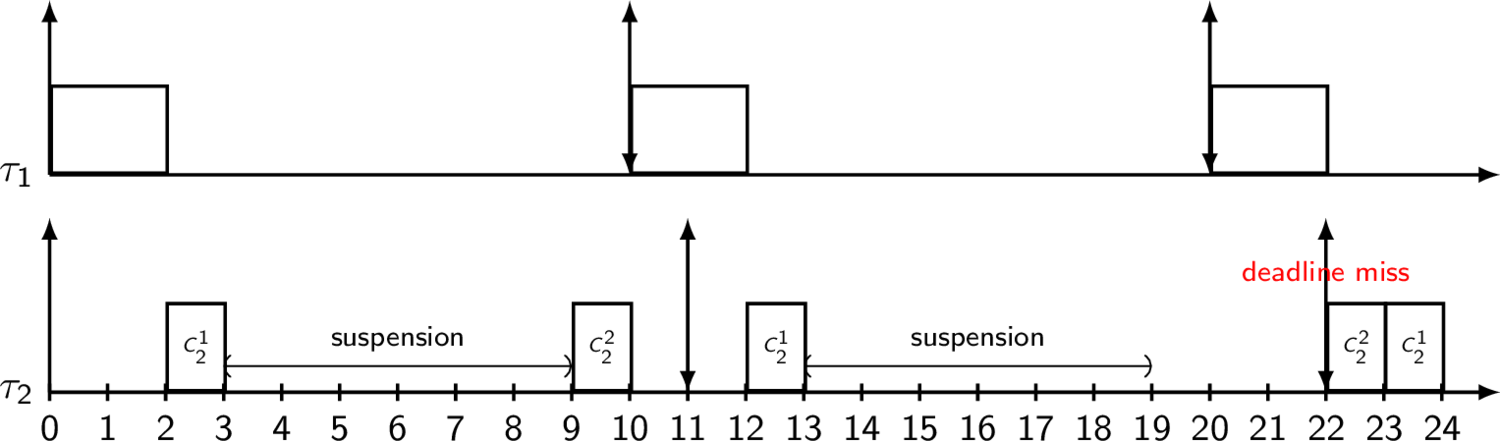
\includegraphics[width=0.9\columnwidth]{figures/example}
\caption{An illustrative example demonstrating a deadline miss at time $22$ under the period enforcer algorithm.
\label{fig:example}%
}
\end{center}
\end{figure}



This example shows that there exist sporadic segmented self-suspending task sets that   \textbf{(i)} are schedulable under fixed-priority scheduling without any enforcement, but \textbf{(ii)} are not schedulable under the period enforcer algorithm.

Furthermore, the example also demonstrates that the conversion to single-segment deferrable tasks does incur a loss of generality since it introduces pessimism: if we convert the two computation segments of task $\tau_2$ into two deferrable tasks $\tau_2^1$ and $\tau_2^2$, where  task $\tau_2^1$ never defers its execution and task $\tau_2^2$ defers its execution by at most \emph{$9$} time units,  then it is immediately obvious that the resulting single-segment deferrable task set $\{\tau_1, \tau_2^1, \tau_2^2\}$ is in fact not schedulable under a rate-monotonic priority assignment since we can time the release of a job of $\tau_1$ to coincide with the arrival of a job of $\tau_2^2$ after it has maximally deferred its execution, which clearly results in a deadline miss.


\clearpage

\section{Deriving a Corresponding Deferrable Task Set}
\label{sec:convert}

The example in Section \ref{sec:unschedulable} can be easily converted to a corresponding single-segment deferrable task set. However, in general,  \emph{precisely} converting a self-suspending task system into a corresponding single-segment  deferrable task set is not an easy problem. We can demonstrate the inherent difficulty by looking at a special case.

Suppose that the system has $k-1$ ordinary sporadic tasks and only one segmented self-suspending task $\tau_k$. Converting a computation segment into a deferrable task requires to derive the \emph{worst-case resume time of a computation segment}, denoted as $R_k^j$ for the $j^{\mathrm{th}}$ computation segment of task $\tau_k$. Suppose that the worst-case response time of the $j^{\mathrm{th}}$ computation segment of task $\tau_k$ is $W_k^j$. It is not difficult to see that $R_k^1=0$ and $R_k^j = W_k^{j-1}+S_k^{j-1}$ for $j=2,3,\ldots,m_k-1$. We therefore need to derive the worst-case response times of the computation segments of task $\tau_k$. 

Based on these considerations, it appears that, at least for the simple example,  the problem is basically identical to the worst-case response time analysis of segmented self-suspending task systems.  However, it has been recently shown by Nelissen et al.\ \cite{ecrts15nelissen} that calculating the worst-case response time in the above ``simple'' case is already a very challenging problem. In particular, Nelissen et al.\ \cite{ecrts15nelissen} identified several misconceptions in prior analyses, and after correcting those misconceptions, observed that deriving the worst-case response time of a computation segment in pseudo-polynomial time seems to be a very challenging problem. 



In the context of the period enforcer, we consequently observe that the only existing solution to derive the \emph{precise} bound $W_k^{j}$ (and hence $R_k^j$), due to Nelissen et al.\ \cite{ecrts15nelissen},  has exponential time complexity (even for the special case above). Furthermore, as demonstrated with the example shown in Figure~\ref{fig:example}, even if the conversion is done precisely, the transformed single-segment deferrable task set can admit more pessimism than the original self-suspending task set with respect to schedulability.

\section{Concluding Remarks}

We have revisited the period enforcer algorithm proposed by Rajkumar \cite{Raj:suspension1991} to handle segmented self-suspending real-time tasks. One key assumption in the original report \cite{Raj:suspension1991} is that a deferrable task $\tau_i$ can defer its entire execution time but not parts of it. This creates some mismatches between the original self-suspending task set and the corresponding deferrable task set, which we have demonstrated with an example that shows that Theorem 5 in \cite{Raj:suspension1991} does not reflect the schedulability of the original self-suspending task system. 


Furthermore, the original report \cite{Raj:suspension1991} left open the question of how to convert a segmented self-suspending task system to a corresponding deferrable task system. Taking into account recent developments~\cite{ecrts15nelissen}, we have observed that such a task set transformation is non-trivial in the general case.  


Nevertheless, Theorem 5 in \cite{Raj:suspension1991} can be useful for handling self-suspending task systems if there exist \emph{efficient} schedulability tests for the corresponding deferrable task systems or the period enforcer algorithm. However, such tests have not been found yet and the development of a precise and efficient schedulability test for self-suspending tasks remains an open problem.

